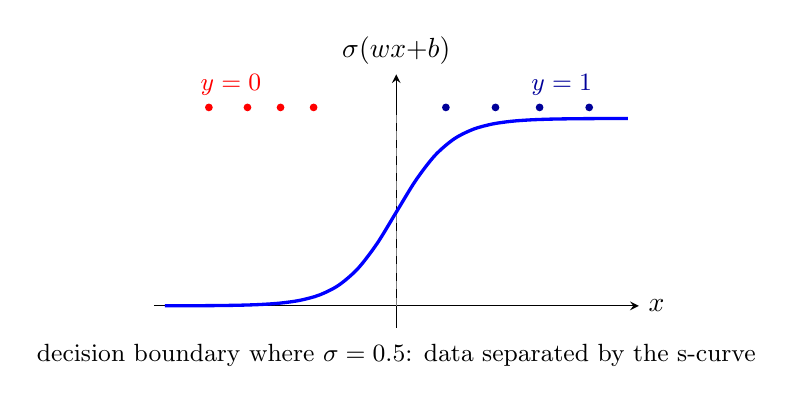
\begin{tikzpicture}[scale=0.7,>=stealth]
\draw[->] (-4.4,0)--(4.4,0) node[right]{$x$};
\draw[->] (0,-0.4)--(0,4.2) node[above]{$\sigma(wx{+}b)$};
\draw[domain=-4.2:4.2,smooth,very thick,blue] plot (\x,{3.4/(1+exp(-2*\x))});
\foreach \x in {-3.4,-2.7,-2.1,-1.5} \fill[red] (\x,3.6) circle (2pt);
\foreach \x in {0.9,1.8,2.6,3.5} \fill[blue!60!black] (\x,3.6) circle (2pt);
\draw[dashed,gray] (0,0)--(0,3.6);
\node[red] at (-3.0,4.0) {\small $y=0$};
\node[blue!60!black] at (3.0,4.0) {\small $y=1$};
\node at (0,-0.9) {\small decision boundary where $\sigma=0.5$: data separated by the s-curve};
\end{tikzpicture}
